\section{Создание графического интерфейса пользователя}
\label{sec:gui}

Для обеспечения удобного взаимодействия оператора с измерительной системой и контроля процесса измерений в реальном времени было разработано специализированное клиентское приложение с графическим интерфейсом пользователя.

К разрабатываемому интерфейсу были сформулированы функциональные требования, указанные ниже.

Управление подключением и настройками: Возможность выбора последовательного порта, к которому подключён микроконтроллер, а также выбора директории и шаблона имени для сохранения файлов с данными.

Двусторонняя коммуникация с МК: Отправка управляющих команд (начало/остановка измерений, перезагрузка) и приём телеметрии в реальном времени.

Визуализация данных: Отображение текущих показаний со всех датчиков (акселерометр, гироскоп) в удобной форме, например, в виде таблицы или простых индикаторов, для оперативной оценки работоспособности системы.

Управление процессом измерений: Предоставление интуитивно понятных элементов управления (кнопки) для запуска и завершения сеанса измерений, а также для выполнения вспомогательных операций, таких как привязка к координатам GPS.

Формирование лога событий: Наличие информационной панели для отображения статусных сообщений, ошибок и подтверждения выполненных действий.


\begin{figure}[ht]
	\centering
	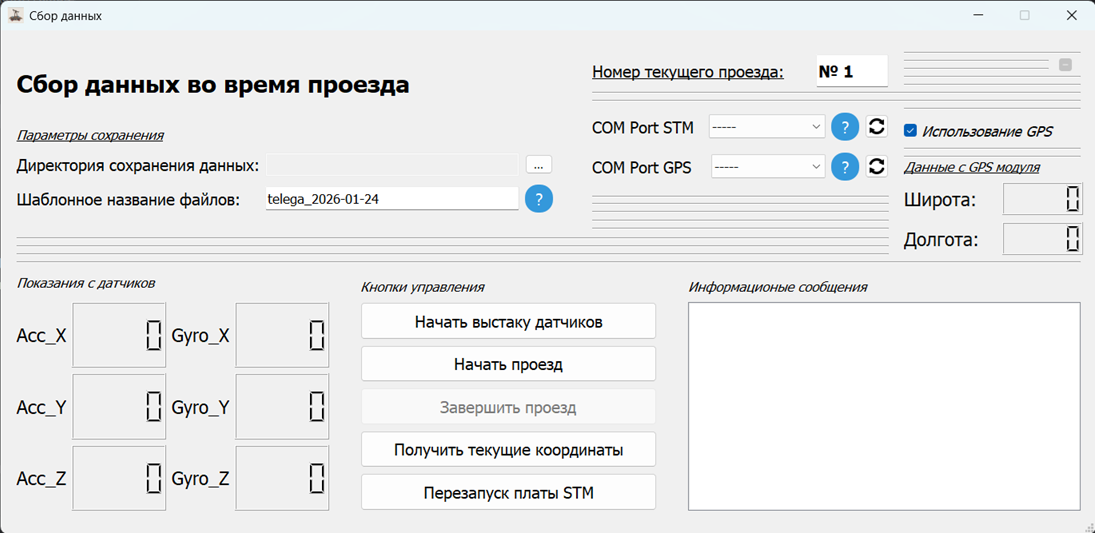
\includegraphics[width=0.9\textwidth]{images/main_part/GUI.png}
	\caption{Разработанный графический интерфейс программы}
	\label{picture:GUI}
\end{figure}

Разработанное приложение, внешний вид которого представлен на рис. \ref{picture:GUI}, полностью удовлетворяет перечисленным требованиям. Его интерфейс логически разделён на несколько функциональных зон:

\begin{itemize}
	\item Секция параметров сохранения (поля для указания пути сохранения данных и шаблона имени файлов, что обеспечивает структурированное хранение результатов каждого проезда);
	\item Секция управления подключением (элементы для выбора COM-портов микроконтроллера и GPS-модуля, а также переключатель активации использования геопозиционных данных);	
	\item Панель визуализации данных в реальном времени (таблица для отображения текущих значений с акселерометра и гироскопа).
	\item Панель управления (группа кнопок для всех ключевых действий: «Начать выставку датчиков» (калибровка), «Начать проезд», «Завершить проезд», «Получить текущие координаты» и «Перезапуск платы STM»);
	\item Область информационных сообщений (Текстовое поле, выполняющее роль лога событий, для вывода служебной информации и диагностики).
\end{itemize}

Приложение реализовано на языке Python с использованием фреймворка PyQt5 для создания производительного и кроссплатформенного графического интерфейса. Выбор PyQt5 обусловлен его мощными возможностями для создания сложных интуитивных интерфейсов, стабильной работой и простой интеграцией с библиотеками для последовательной связи (PySerial) и научных вычислений (NumPy), что в совокупности обеспечило требуемую функциональность и надёжность.




